\documentclass[a4paper,kulak]{kulakarticle}

\usepackage[utf8]{inputenc}
\usepackage[dutch]{babel}
\usepackage{pdfpages}
\usepackage{subfig}
\usepackage{float}

\usepackage{cite}

% style
%\usepackage[left=2.5cm,top=2cm,right=2.5cm,bottom=2cm,a4paper]{geometry}
\usepackage{color}

\date{\today}
\address{
	Bachelor in de fysica\\
	Bachelor in de informatica\\
	Bachelor in de wiskunde\\
	Ingenieurswetenschappen}
\title{BDA App}
\author{Marthe B\"{o}ting, Robin Bruneel en Toon Ingelaere}

\begin{document}
	\includepdf{voorblad}
	%\newpage
	
	\maketitle
	\section*{Inleiding}
		Beroertes zijn in onze westerse samenleving de derde grootste doodsoorzaak na hartinfarcten en kanker. Zoals we zien op Figuur \ref{figuur doodsoorzaken} kapen ze op wereldvlak zelfs de tweede plaats weg\cite{worldhealthorganization}. In België komen er gemiddeld 25 000 beroertes per jaar voor. In 15\% van deze gevallen overlijdt de patiënt. De overige 85\% heeft na een beroerte vaak last van blijvende functiebeperkingen zoals cognitieve-, emotionele of gedragsproblemen. Een ischemische beroerte ontstaat doordat een bloedklonter emboliseert en in één van de hersenbloedvaten vast komt te zitten. Deze bloedklonter moet verwijderd worden of de patiënt loopt een hersenschade op.
		Momenteel focust de huidige therapie zich op snel en efficiënt verwijderen van de bloedklonter. In eerste instantie kan men via een geneesmiddel, weefsel plasminogeen activator, proberen om de klonter op te lossen. Dit geneesmiddel moet gegeven worden binnen de eerste 4,5 uur na het optreden van de symptomen. Wanneer dit geneesmiddel wordt toegediend na dit tijdstip kan dit leiden tot bloedingen of toxiciteit in de hersenen. Van alle patiënten die het geneesmiddel toegediend krijgen, lost de klonter slechts in 1/3 van de patiënten op.
		Op het moment dat de klonter niet oplost , maakt men gebruik van trombectomie om de klonter er manueel uit te halen.
		Om huidige therapeutische opties te verbeteren en om het aantal slachtoffers aan beroertes te doen slinken, gebruikt men deze bloedklonters om verder onderzoek op uit te voeren. Hiervoor gaan ze de samenstelling van de bloedklonter proberen te analyseren. Dit gebeurt op basis van afbeeldingen die gemaakt zijn van de bloedklonter waarbij welbepaalde componenten gekleurd zijn (bijvoorbeeld: rode bloedcellen, witte bloedcellen en bloedplaatjes) en vervolgens geanalyseerd worden via kleur-gebaseerde segmentatie analyse.
		Deze analyses zijn echter erg tijdrovend. Er is ons dan ook gevraagd om een gebruiksvriendelijke app te ontwikkelen die de analyse van de afbeeldingen kan automatiseren.
		In dit verslag gaan we eerst in op wat de klant specifiek van ons verwacht en aan welke specificaties ons ontwerp moet voldoen. Hierna bespreken we ons design en lichten we het toe. Verder bespreken we ook enkele van onze voorlopige resultaten. Ten slotte wordt er nog een blik geworpen naar de vakken uit eerste drie semesters die ons hierbij geholpen hebben.

\begin{figure}[H]
	\centering
	\includegraphics[width = 0.7\textwidth]{top10doodsoorzaken.png}
	
	\caption{Statistieken van de \textit{World Health Organization} van 2016 waarin te zien is dat wereldwijd beroertes (\textit{strokes}) de tweede meest frequente doodsoorzaak is.}
	\label{figuur doodsoorzaken}
\end{figure}

\tableofcontents

\section{Klantenvereisten}
De klant verwacht een gebruiksvriendelijke app die de afbeeldingen automatisch verwerkt. Dit houdt in dat een afbeelding ingeladen kan worden, de foto bijgesneden en de achtergrond verwijderd worden. Daarnaast is het de bedoeling om de samenstelling van de bloedklonter te analyseren aan de hand van de aangebrachte indicator.

\section{Ontwerpspecificatie}
De klant wil dat een afbeelding van een bloedklonter automatisch bewerkt en daarna geanalyseerd wordt.\\
Het bewerken van de afbeelding houdt twee dingen in. Eerst en vooral moet de afbeelding zodanig bijgesneden worden dat de volledige bloedklonter erop staat. Hierbij mogen we de randen echter niet te breed nemen, aangezien er dan nuttige geheugenruimte\footnote{We werken namelijk met foto's van de orde van 200MB, het sparen van pixels op ons resultaat is uiterst voordelig} verspild wordt. 
Naast het bijsnijden, moet ook de achtergrond verwijderd worden. Dit betekent dat alle pixels die niet tot de bloedklonter behoren wit gekleurd worden. Indien dit niet goed gebeurt, kunnen de resultaten van de kleurenanalyse namelijk vertekend zijn.\\
In de kleurenanalyse moet het percentage van met indicator gekleurde pixels geteld worden. Voor dit project moeten we slechts twee soorten kleuringen analyseren. Een voorbeeld van deze is te zien in Figuur \ref{figuur indicators}. In beide gevallen moet de app op een accurate manier onderscheid kunnen maken tussen de eiwitten die gedetecteerd moeten worden en de rest van de bloedklonter. \\
Dit alles moet samengegoten worden in een visuele en gebruiksvriendelijke app. Dit wil zeggen dat de app makkelijk te installeren en te gebruiken is. De gebruiker moet ook een overzicht van de verschillende afbeeldingen van de bloedklonter kunnen terugroepen. Dit overzicht bestaat uit de originele afbeelding, de afbeelding zonder achtergrond en de afbeelding waarbij de indicatorpixels zijn aangeduid. Zo kunnen mogelijke fouten snel gedetecteerd worden. Indien gewenst kan deze app nog heel wat extra functionaliteiten uitvoeren zoals het opslaan van deze afbeeldingen, het wegschrijven van alle data in een csv\footnote{Een csv (Comma Separated Values) bestand is een tekstbestand die als tabel ingelezen kan worden. Het kan eenvoudig in excel geopend worden voor verdere analyse.} bestand, etc.

\section{Onze oplossing}
Dit hoofdstuk is opgedeeld in verschillende deelproblemen: het verwijderen van de achtergrond, het lokaliseren van de indicator en de gebruiksvriendelijke app. De app is gerealiseerd met behulp van de programmeertaal MATLAB.

\subsection{Achtergrondverwijdering}
Het eerste deelprobleem van ons project is het verwijderen van de achtergrond. Op de afbeeldingen is er heel wat vuiligheid te vinden. Voorbeelden hiervan zijn luchtbellen of kleine verkleuringen in de achtergrond zoals men ziet op de Figuur \ref{figuur achtergrondverwijdering}. Hieronder beschrijven we verschillende operaties om de grootste klonters te lokaliseren en alles wat geen klonter is te verwijderen. Dit leidt tot een ruisvrije afbeelding.

\begin{figure}[H]
	\centering
	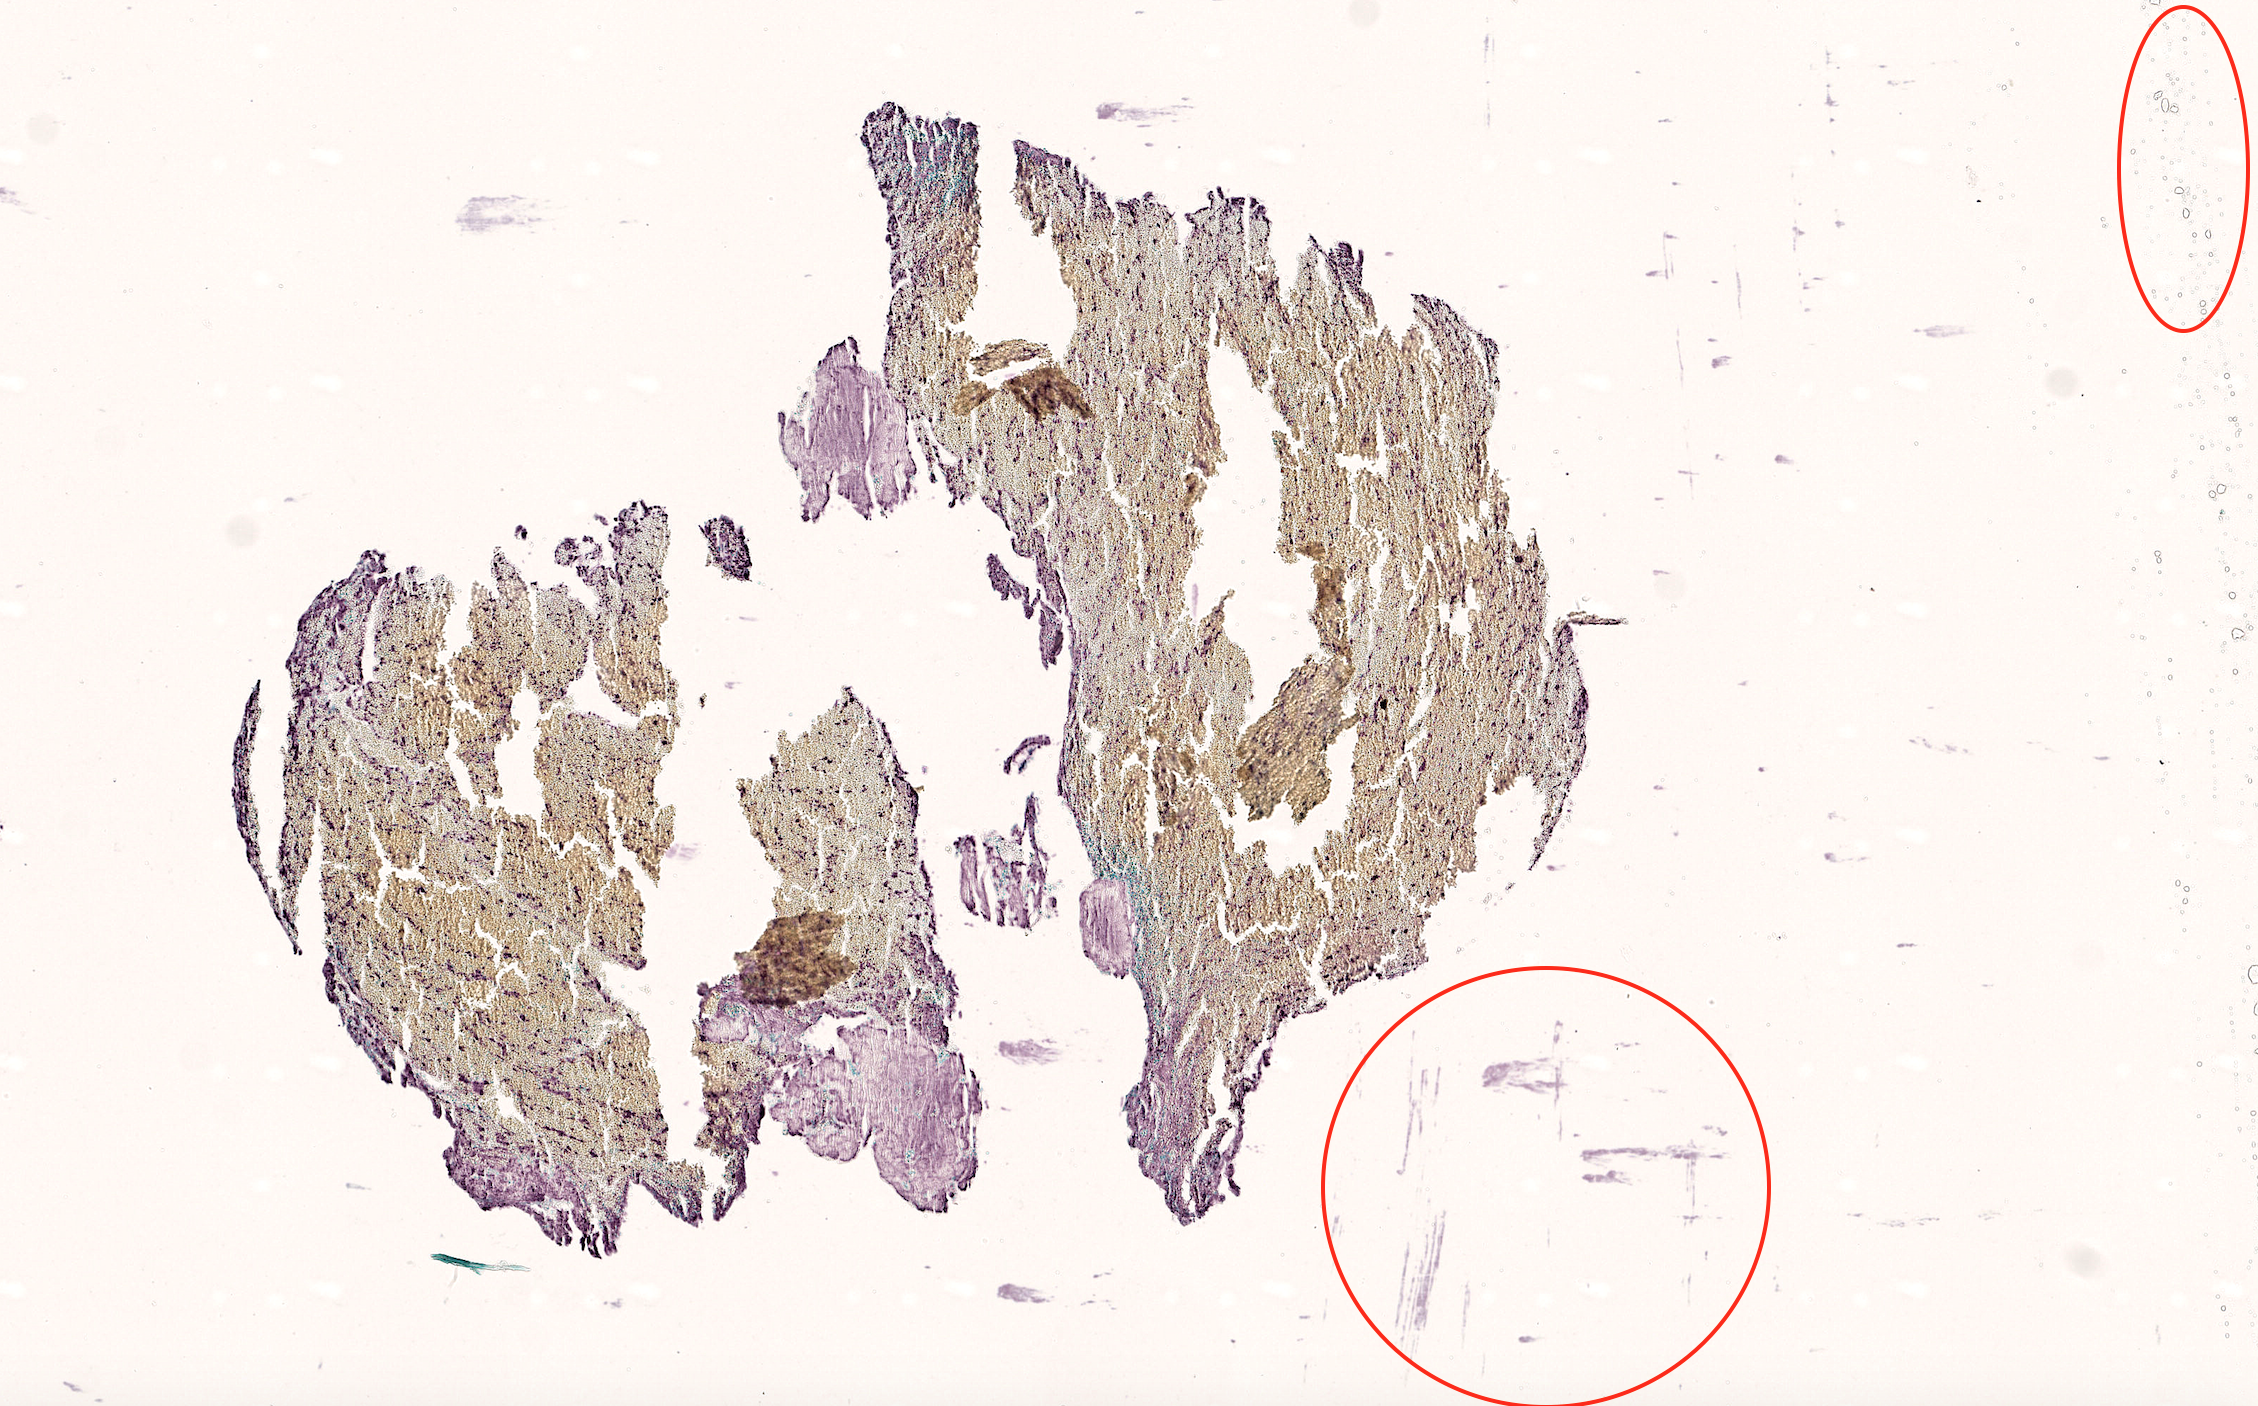
\includegraphics[width = 0.7\textwidth]{Ruis_afbeelding.png}	
	\caption{In de rechterbovenhoek zien we luchtbellen en in de onderste cirkel zien we een verkleuring die geen deel uitmaakt van een bloedklonter.}
	\label{figuur achtergrondverwijdering}
\end{figure}

\subsubsection{Bepalen van de beste threshold}
Het onderscheid tussen de achtergrond (eerder wit) en de bloedklonter (eerder grijs) is makkelijker te zien op de grijswaarden van de afbeelding, zie Figuur \ref{figuur beste_threshold}.. Daarnaast is één grijswaarde voldoende om het onderscheid te maken. Wanneer een histogram opgesteld wordt van deze waarden is een duidelijk dipje tussen het wit en het grijs te zien, zie Figuur \ref{figuur graf1}. Dit is dan ook de theoretisch optimale threshold, de grijswaarde om een bloedklonterpixel van een achtergrondpixel te onderscheiden. Deze bepalen we simpelweg als het minimum in de tweede helft van de histogram. Na het toepassen van de threshold komt de binaire Figuur \ref{figuur foto_bin} tevoorschijn. Dit lijkt de klonters nagenoeg goed te detecteren.

\begin{figure}[H]
	\centering
	\subfloat[]{{\includegraphics[width=6cm]{origineel_vb}}}
	\qquad
	\subfloat[]{{\includegraphics[width=6cm]{grijswaarden_vb}}}
	
	\caption{Illustratie van de originele foto (a) en deze omgezet in grijswaarden (b).}
	\label{figuur beste_threshold}
\end{figure}

\begin{figure}[H]
	\centering
	\includegraphics[width=0.85\textwidth]{GetBestthreshold_vb_aangeduid.png}
	
	\caption{Histogram van het aantal pixels gegroepeerd per grijswaarde. We zien duidelijk een lokaal minimum rond de waarde 230. Opmerking: we maken hier gebruik van een logaritmische y-as.}
	\label{figuur graf1}
\end{figure}

\begin{figure}[H]
	\centering
	\includegraphics[width=0.7\textwidth]{grijswaarden_bin_vb}
	\caption{Op deze binaire representatie zijn de bloedklonters duidelijk te zien.}
	\label{figuur foto_bin}
\end{figure}

\subsubsection{Ruisfilter}
Eenmaal de binaire representatie is opgesteld, kunnen de bloedklonters nauwkeurig gelokaliseerd worden door al het overbodige ruis te verwijderen. De ruis kan makkelijk verwijderd worden door alle kleine groepen witte/zwarte pixels respectievelijk te vervangen door zwarte/witte pixels. Het resultaat is te zien op Figuur \ref{figuur ruisfilter} (a). \\
Deze zogenaamde 'mask'\footnote{Bij het toepassen van een mask op een afbeelding, worden alle pixels in de afbeelding die zwart zijn in de mask, wit gemaakt. De andere pixels behouden hun kleur.} kan toegepast worden op de originele afbeelding om de ruisvrije afbeelding te vormen. Daarnaast wordt deze afbeelding bijgesneden om kostbare geheugenruimte te sparen, zoals te zien is in Figuur \ref{figuur ruisfilter} (b). In dit deelprobleem werd echter met een reeds bijgesneden bloedklonter gewerkt om de afbeeldingen duidelijk te houden. Een volledig onbewerkte afbeelding is echter te zien in Figuur \ref{figuur volledig_onbewerkt}

\begin{figure}[H]
	\centering
	\subfloat[]{{\includegraphics[width=7cm]{ruisvrij_vb}}}
	\qquad
	\subfloat[]{{\includegraphics[width=7cm]{ruisvrij_kleur_vb}}}
	
	\caption{Alle ruis is verwijderd, dit is een foto waarmee we kunnen werken.}
	\label{figuur ruisfilter}
\end{figure}

\begin{figure}[H]
	\centering
	\includegraphics[width=15.25cm]{Volledig_onbewerkt}
	
	\caption{Dit is een volledig onbewerkte afbeelding die we in \ref{figuur ruisfilter} (b) hebben bijgesneden en waarvan de achtergrond verwijderd is.}
	\label{figuur volledig_onbewerkt}
\end{figure}
\subsection{Lokalisatie van de indicator}
Het tweede deel van ons project is de indicators lokaliseren en kwantificeren. We hebben de opdracht gekregen twee soorten te kunnen onderscheiden. Van deze is een voorbeeld op Figuur \ref{figuur indicators} te zien. Omdat het kleurverschil tussen indicator en achtergrond niet altijd even groot is, vormen we het oorspronkelijke \textit{RGB} kleurmodel\footnote{Het RGB kleurmodel is een voorstelling waarbij ieder kleur voorgesteld wordt door een waarde van de drie basiskleuren (rood, groen en blauw)} om naar het zogenaamde \textit{HSV} kleurmodel. Dit model is een alternatieve voorstelling waarbij men alle kleuren op een cirkel voorstelt, de hoek die dit kleur dan maakt, noemt men de \textit{Hue}. Naast deze waarde heeft \textit{HSV} nog twee andere parameters namelijk \textit{Saturation} en \textit{Value}. \textit{Saturation} kan simpel beschouwd worden als een aanduiding van de hoeveelheid witte kleur en \textit{Value} een aanduiding van de zwarte kleur. Een grafische voorstelling is te zien op Figuur \ref{figuur hsv_schema}.\\
Het voordeel van deze transformatie is dat het heel wat eenvoudiger is om een onderscheid tussen dichtbijgelegen kleuren te vinden. Een andere mogelijke transformatie is die naar het \textit{Lab} kleurmodel die gelijkaardige eigenschappen heeft en desnoods ook gebruikt kan worden. Eenmaal we een duidelijk onderscheid tussen de indicator en de achtergrond maken, kunnen we eenvoudig het percentage indicator berekenen door het aantal bloedklonter- en indicatorpixels op te tellen. Ons stappenplan wordt in volgende hoofdstukken besproken en wordt toegepast op de afbeelding uit Figuur \ref{figuur indicators} (a).

\begin{figure}[H]
	\centering
	\subfloat[]{{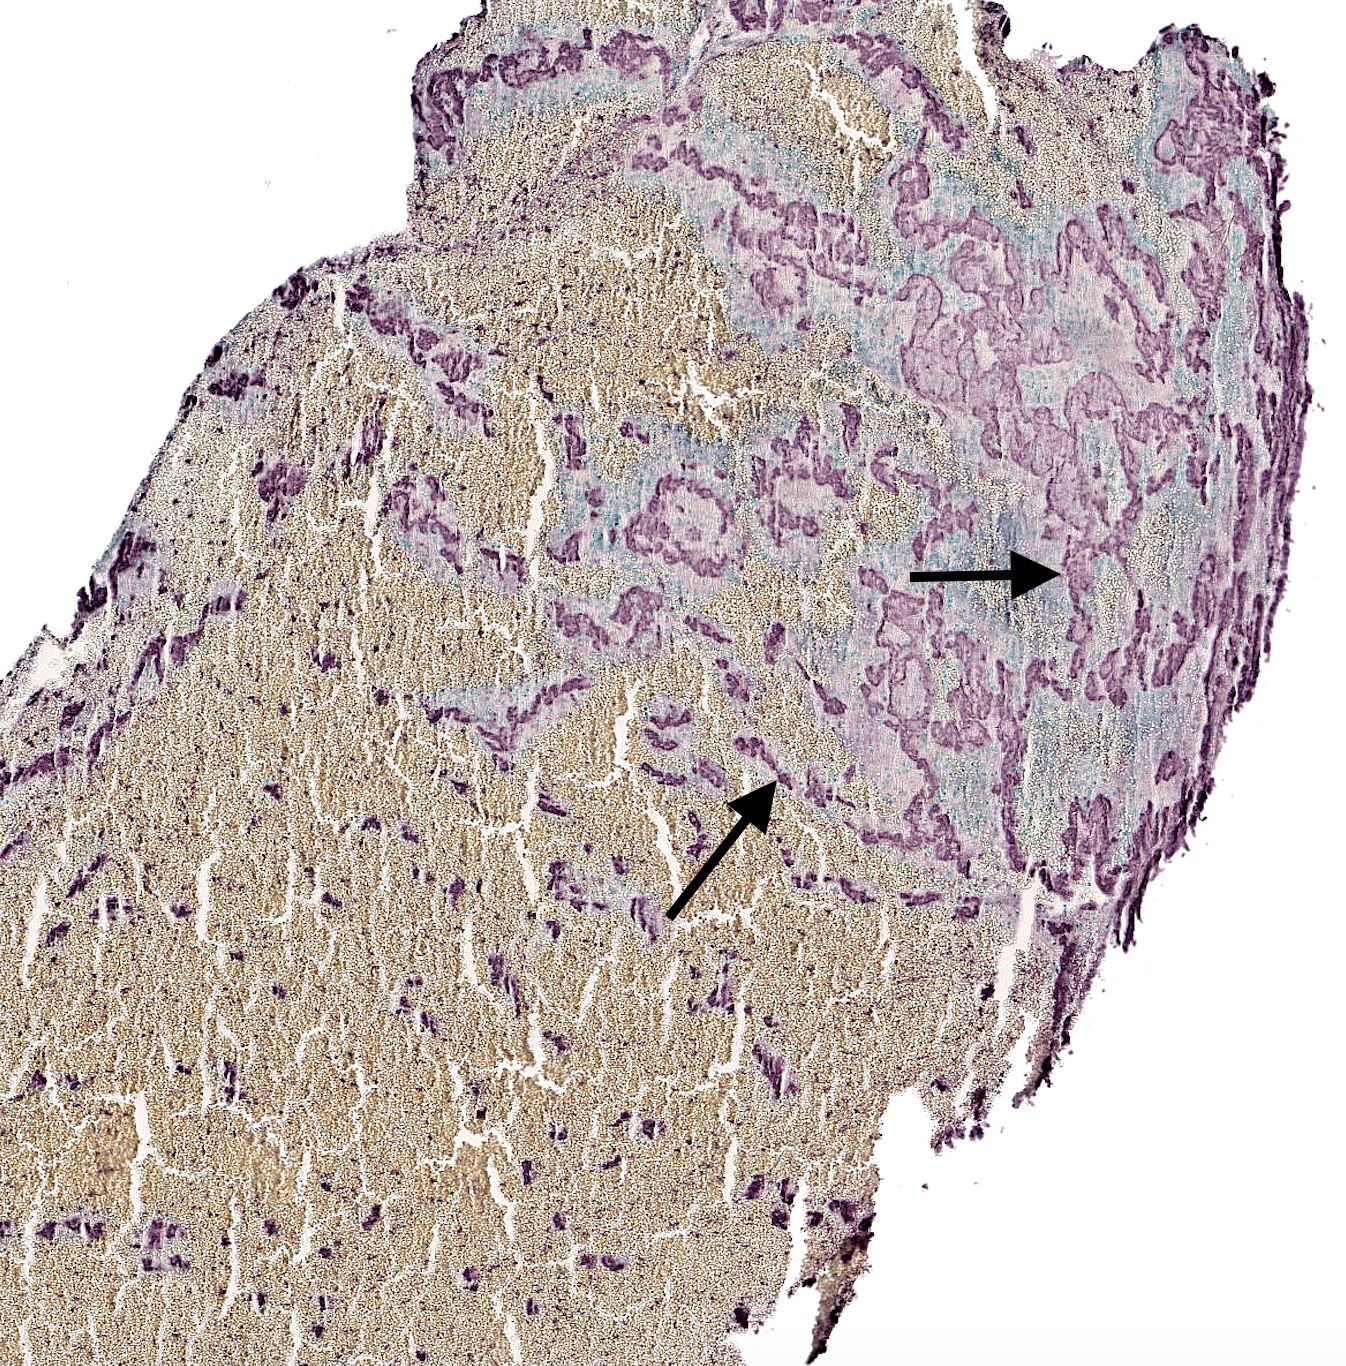
\includegraphics[width=7cm]{Indicator_vb1}}}
	\qquad
	\subfloat[]{{\includegraphics[width=7cm]{Indicator_vb2}}}
	
	\caption{Illustratie van de twee soorten indicator (respectievelijk paars en donkerroze) die gedetecteerd moeten worden. We zien duidelijk dat het detecteren op afbeelding (a) eenvoudiger zal zijn dan op afbeelding (b).}
	\label{figuur indicators}
\end{figure}

\begin{figure}[H]
	\centering
	\includegraphics[width=0.7\textwidth]{HSV_vb.png}
	
	\caption{Grafische voorstelling van het \textit{HSV} (\textit{Hue}, \textit{Saturation}, \textit{Value}) kleurmodel}
	\label{figuur hsv_schema}
\end{figure}

\subsubsection{Het HSV kleurmodel}
Zoals reeds vermeld, beginnen we met een transformatie naar het \textit{HSV} kleurmodel. Bijgevolg kunnen we de twee voorstellingen vergelijken. We hebben het model telkens ontbonden in de drie kleurwaarden, waarbij zwart de laagste waarde voor dat kleur is en wit de hoogste. De resultaten zijn te zien in de Figuren \ref{figuur RGB} en \ref{figuur HSV}. Het verschil tussen de twee kleurmodellen is duidelijk te zien. Afbeelding (a) en (b) uit Figuur \ref{figuur HSV} lijken namelijk een iets agressiever onderscheid te maken.

\begin{figure}[H]
	\centering
	\subfloat[]{{\includegraphics[width=4.5cm]{RGB_r}}}
	\qquad
	\subfloat[]{{\includegraphics[width=4.5cm]{RGB_g}}}
	\qquad
	\subfloat[]{{\includegraphics[width=4.5cm]{RGB_b}}}
	\caption{Illustratie van respectievelijk de rode, groene en blauwe kleurwaarden (\textit{RGB}). Hierbij komt wit overeen met de maximumwaarde en zwart met de minimumwaarde van die kleur.}
	\label{figuur RGB}
\end{figure}

\begin{figure}[H]
	\centering
	\subfloat[]{{\includegraphics[width=4.5cm]{HSV_h}}}
	\qquad
	\subfloat[]{{\includegraphics[width=4.5cm]{HSV_s}}}
	\qquad
	\subfloat[]{{\includegraphics[width=4.5cm]{HSV_v}}}
	
	\caption{Illustratie van respectievelijk de \textit{hue}, \textit{saturation} en \textit{value} kleurwaarden (\textit{HSV}). Hierbij komt wit overeen met de maximumwaarde en zwart met de minimumwaarde van die kleurwaarde.}
	\label{figuur HSV}
\end{figure}

\subsubsection{Een algemene threshold}
De volgende stap is nu een filter bepalen voor alle indicatorpixels. Het probleem is echter dat een goede filter voor de ene foto niet altijd een goede filter voor de andere foto is. Daarom hebben we voor iedere foto manueel een 'threshold' bepaald en deze achteraf met elkaar vergeleken. Het resultaat is een vrij algemene threshold die alle indicatorpixels met zekerheid aanduidt. Af en toe worden jammer genoeg verkeerde pixels aangeduid. Het aantal is weliswaar niet zo groot, maar dit zullen we trachten te omzeilen in het volgende hoofdstuk. Een voorbeeld van deze algemene threshold is te zien op de Figuur \ref{figuur alg_tresh}.
\begin{figure}[H]
	\centering
	\includegraphics[width = 0.7\textwidth]{algemene_threshold}
	
	\caption{We hebben alle indicatoren met een blauwe kleur aangeduid. De algemene threshold selecteert alle indicatorpixels, maar jammer genoeg ook enkele verkeerde (voornamelijk rechtsonder).}
	\label{figuur alg_tresh}
\end{figure}

\subsubsection{Optimalisatie van de threshold}
In dit hoofdstuk willen we het aantal verkeerde pixels verminderen zonder de juiste te beïnvloeden. We hebben echter al een vrij goede threshold waardoor we een statistische analyse van wat onder deze mask ligt, kunnen uitvoeren. We stellen hiervoor een frequentiediagram van de \textit{HSV} kleurwaarden onder de mask op. Het levert ons namelijk een interessant resultaat dat te zien is in Figuur  \ref{figuur HSVHIST}. We zien namelijk duidelijke verschillen in de frequenties van de kleurwaarden. De grafieken tussen de verschillende afbeeldingen zijn nagenoeg gelijk van vorm, maar de pieken liggen soms meer dan 5\% verschoven.\\
Het idee is om nu de verkeerde pixels via deze diagrammen eruit te filteren. Indien we veronderstellen dat de frequenties van deze specifieke pixels laag zijn en dat de verkeerde pixels in kleur verschillen met de indicatorpixels. Dan kunnen we in principe alle pixels met een frequentie onder een bepaalde grenswaarde schrappen. Een betere benadering is misschien om het punt te vinden, waar de frequentie van de pixels enorm begint toe te nemen of we met andere woorden grote 'indicatoraders' aan het verwijderen zijn. Dit punt kan theoretisch benaderd worden als het maximum van de tweede afgeleide naar de kleurwaarde. Jammer genoeg hebben we de tijd nog niet gehad om dit idee toe te passen. \\
Een mogelijk extra stap is om de indicatorpixels morfologisch te sluiten met een algoritme dat reeds in MATLAB verwerkt is. Indien we met onze filtering enkele holtes maken, kunnen deze dan zonder problemen worden opgevuld. Ter illustratie geven we het standaardvoorbeeld van MATLAB in Figuur \ref{figuur morf} weer.


\begin{figure}[H]
	\centering
	\subfloat[]{{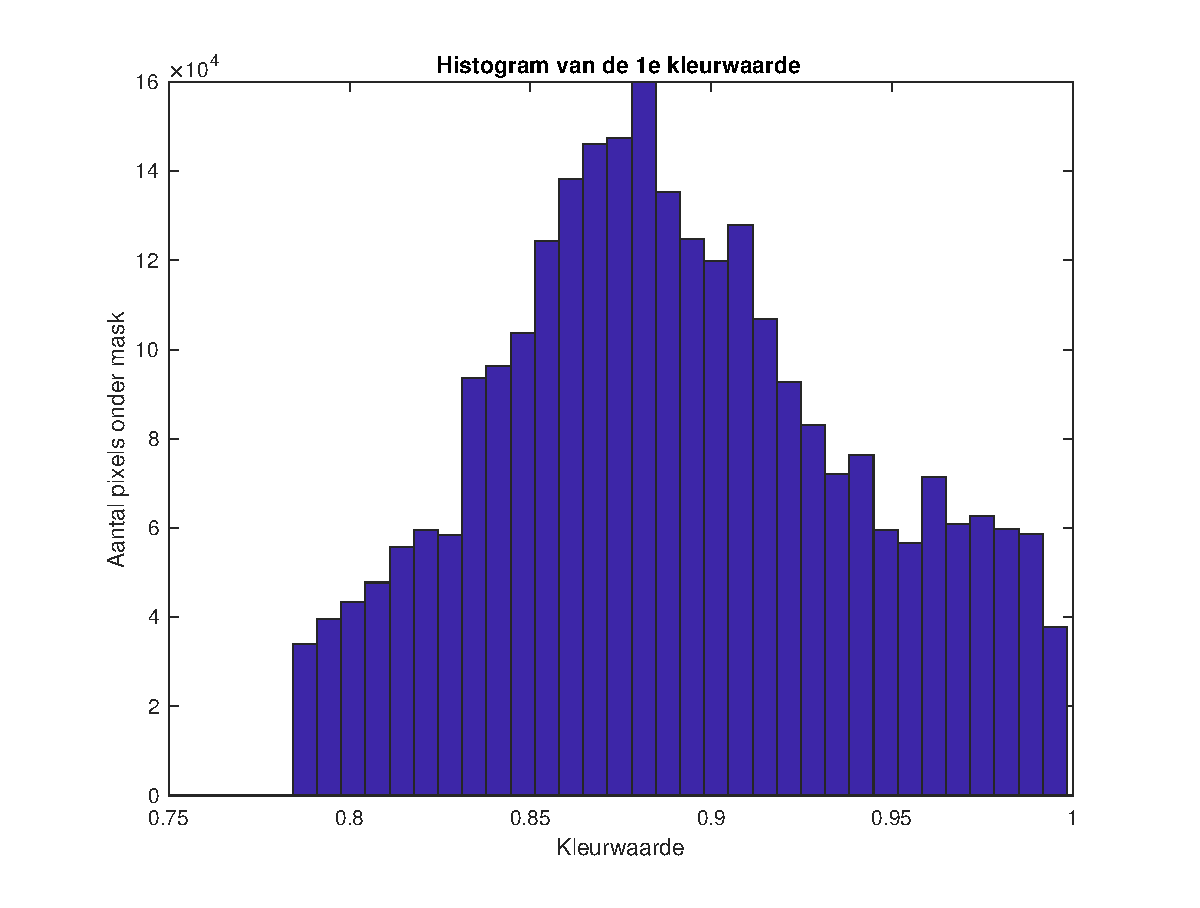
\includegraphics[width=4.5cm]{hsvhist_h}}}
	\qquad
	\subfloat[]{{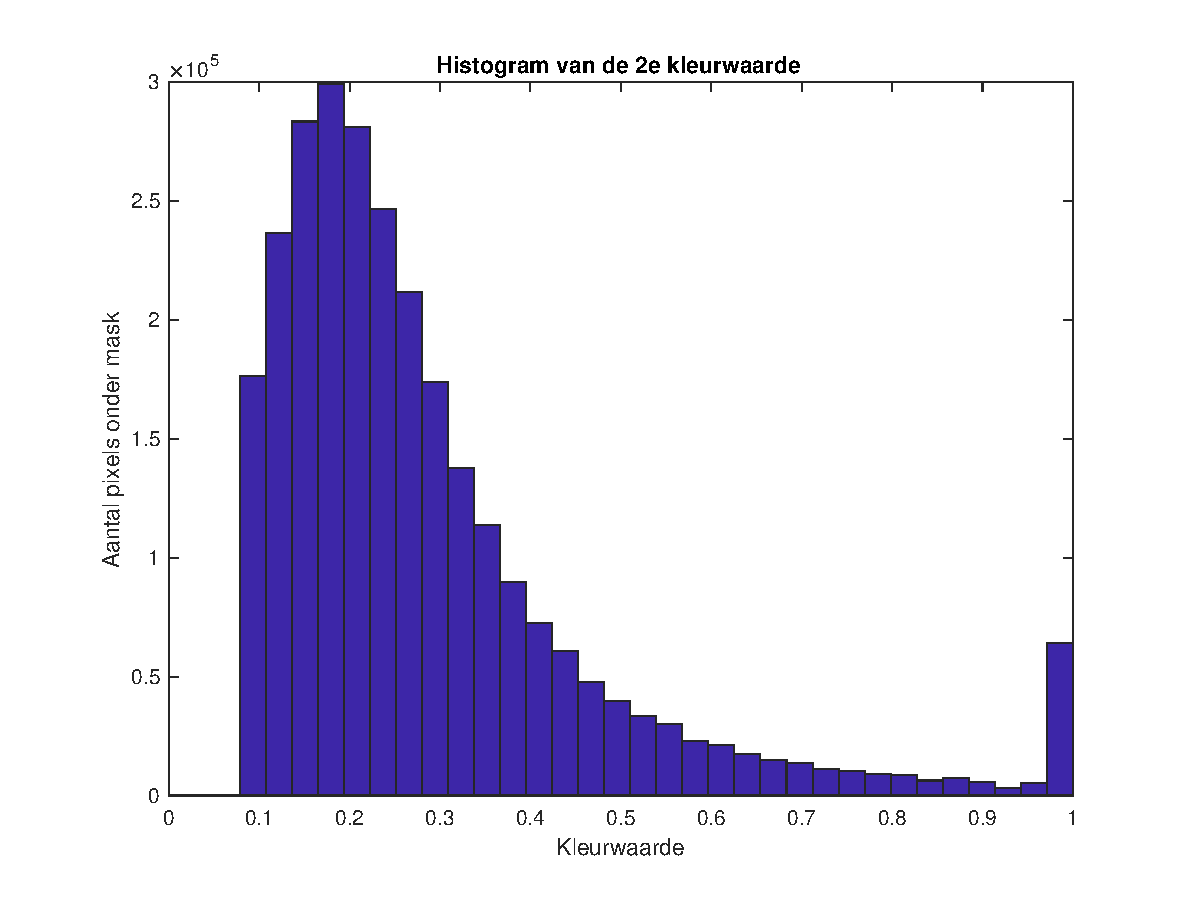
\includegraphics[width=4.5cm]{hsvhist_s}}}
	\qquad
	\subfloat[]{{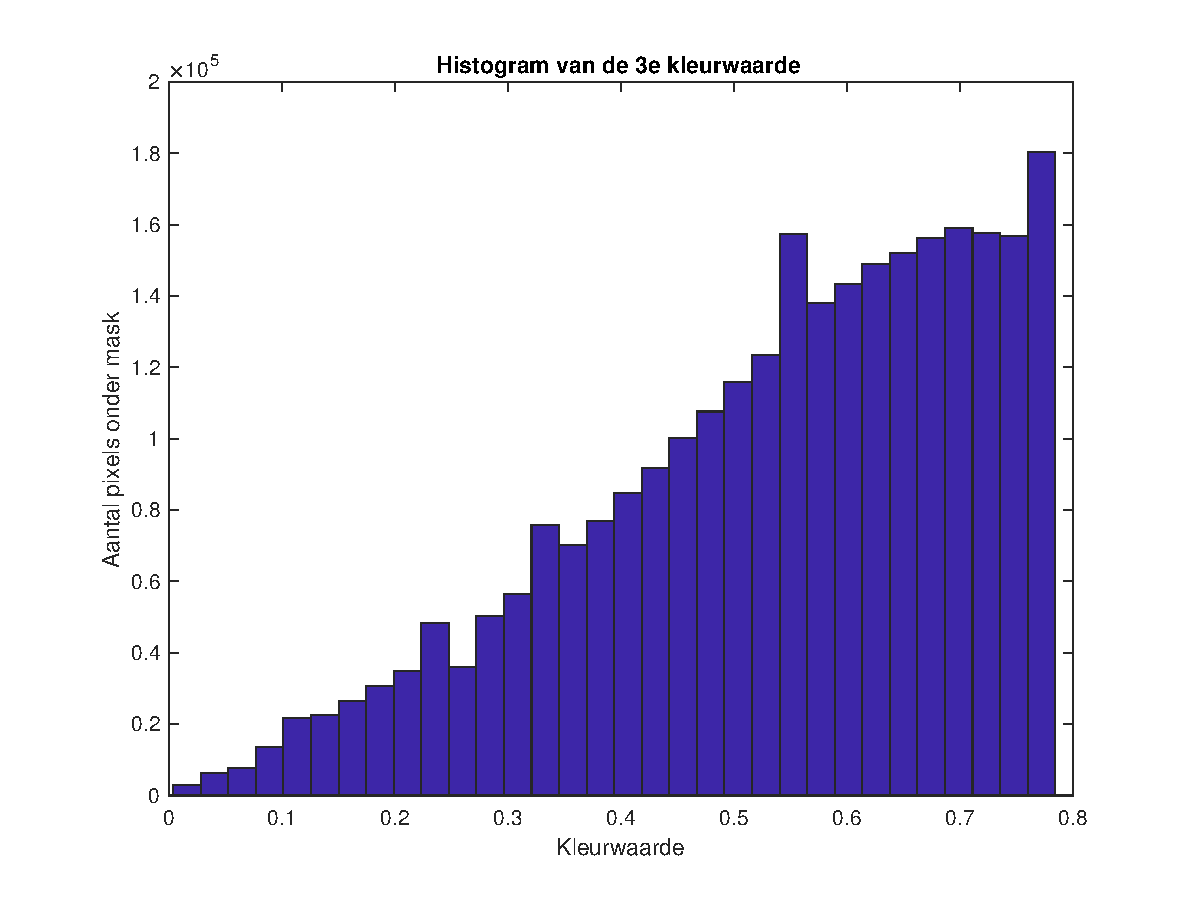
\includegraphics[width=4.5cm]{hsvhist_v}}}
	
	\caption{Histogrammen van de HSV kleurwaarden. We zien duidelijk het verschil in frequenties.}
	\label{figuur HSVHIST}
\end{figure}

\begin{figure}[H]
	\centering
	\subfloat[]{{\includegraphics[width=7cm]{morf_open}}}
	\qquad
	\subfloat[]{{\includegraphics[width=7cm]{morf_gesloten}}}
	
	\caption{Illustratie waarbij de witte cirkels uit afbeelding (a) morfologisch gesloten worden in afbeelding (b)}
	\label{figuur morf}
\end{figure}

\subsection{De gebruiksvriendelijke applicatie}
Momenteel hebben we nu nog enkel afzonderlijke programma's waarbij we steeds zelf de bestandslocatie van de aan te passen foto in de code moeten schrijven. Naar de klant toe is dit geen manier van werken en dienen deze programma's in een app samengebracht te worden. De klant zal dan zelf kunnen ingeven welke foto hij wil laten verwerken. Eénmaal de foto gekozen is, zal in de eerste fase de achtergrond van de foto wit worden gemaakt en zal de foto bijgesneden worden zodanig dat enkel de bloedklonter zichtbaar is. Als dit gebeurd is, zal er al een eerste resultaat getoond worden. Hierdoor heeft de klant een beeld waarop de verdere analyse zal gebeuren en kan die eventueel ingrijpen bij fouten. Vervolgens zal de kleurenanalyse gebeuren. Ook hiervoor zal de foto getoond worden waarop de klant kan zien welke delen de indicator bevatten en zal het percentage gegeven worden. De basis lay-out van de app hebben we al; zoals te zien is in Figuur \ref{fig: app}.

\begin{figure}[H]
	\centering
	\includegraphics[width=170mm]{app.jpg}
	\caption{Voorlopige lay-out van de app.}
	\label{fig: app}
\end{figure}




\section{Voorlopige resultaten}		
Momenteel kunnen we een afbeelding gebruiksklaar maken voor de analyse ervan. Dit houdt in dat we alle pixels die niet tot de bloedklonter behoren wit kunnen maken en de afbeelding zodanig bijsnijden dat er geen overbodig geheugen door de afbeelding ingenomen wordt. In Figuur \ref{fig: voorna} wordt dit geïllustreerd.\\

\begin{figure}[H]
	\centering
	\subfloat[Afbeelding van bloedklonter voor die bewerkt wordt]{{\includegraphics[width=7cm]{BloedklonterVoor.jpg}}}
	\qquad
	\subfloat[Bijgesneden afbeelding van de bloedklonter met witte achtergrond ]{{\includegraphics[width=7cm]{BloedklonterNa.jpg}}}
	
	\caption{Illustratie van hoe we de afbeelding gebruiksklaar maken voor de analyse ervan}
	\label{fig: voorna}
\end{figure}


Daarnaast zijn we bezig met de implementatie van de kleurendetectie. We hebben hier al veel vooruitgang geboekt, maar de hij staat nog niet volledig op punt. Ook hebben we al even geëxperimenteerd met de 'app designer' van MATLAB. Hier willen we namelijk onze gebruiksvriendelijke applicatie in programmeren.\\
Aangezien we de afbeeldingen met de oranje kleuringen nog maar recent ontvangen hebben, hebben we met deze ook nog niet geëxperimenteerd.\\
Op basis van wat we nu al bereikt hebben, denken we dat dit project een succes kan worden en dat men het effectief zal kunnen gebruiken in het onderzoek naar de samenstelling van bloedklonters.

\section{Verantwoordelijkheden en taakverdeling}		
In onze groep hebben we ervoor gekozen om Robin aan te stellen als projectleider. Hij verdeelt elke week de taken en heeft het laatste woord bij discussies. 
Voor de verslagen en de eindpresentatie is Marthe verantwoordelijk. Zij is de eindredactrice van alle verslagen. We schrijven deze uiteraard samen, maar het is haar taak ervoor te zorgen dat deze volledig en gestructureerd zijn en dat ze voor de deadline ingediend worden.\\
Voor de implementatie van de code zijn we elk verantwoordelijk voor ons eigen deel. Zo wordt het verwijderen van de ruis en het bijsnijden van de afbeelding door Toon geleid, de kleurdetectie door Robin en de implementatie van de app door Marthe.\\
Helemaal achteraan dit verslag voegden we ook een Gantt-chart toe. Hierin staan enkele belangrijke deadlines vermeld en onze voorlopige planning. We hebben het project opgesplitst in vier verschillende taken die we elk ingepland hebben zoals afgebeeld. Ook de tijd die we rekenen voor het tussentijds - en het finaal verslag, zijn af te lezen in de chart.

\section{Integratie van vakken}
Om dit probleem op te lossen, hebben we gebruik gemaakt van MATLAB. Het is dan ook een meerwaarde dat we in het eerste semester het vak 'Beginselen van Programmeren' gehad hebben om sneller vertrouwd te raken met deze nieuwe programmeertaal. Daarnaast leren we ook in 'nummerieke wiskunde' werken met MATLAB. Om de verschillende thresholds te bepalen in ons programma, maken we ook gebruik van en statistische analyse van de pixelwaarden. Het vak 'Statistiek' draagt hier dus ook zijn steentje bij.

\section{Besluit}	
Momenteel kunnen we besluiten dat we goed aan het vorderen zijn. Zoals eerder vermeld kunnen we de foto automatisch bijsnijden en de achtergrond ruisvrij maken. Onze focus ligt nu voornamelijk bij de implementatie van de kleurendetectie. Eénmaal deze ook op punt staat kunnen we beide programma's in de app steken en deze optimaliseren met de nadruk op gebruiksvriendelijkheid naar de klant toe. Verder houden we de klant op de hoogte over onze vooruitgang via onder andere dit verslag. 
	
	
	\includepdf[page={1-3}]{ganttchart}	
	
	

\end{document}
